\documentclass[t]{beamer}
\usepackage{mathtools}
\usepackage{tikz}
\usepackage{pgfplots}
\usetikzlibrary{arrows,backgrounds,shapes,matrix,positioning,fit}
\newcommand{\argmax}{\operatornamewithlimits{argmax}}
\newcommand{\argmin}{\operatornamewithlimits{argmin}}
\newcommand{\wt}{\operatornamewithlimits{wt}}
\newcommand{\var}{\operatornamewithlimits{var}}

\mode<presentation>
{
  \usetheme{Singapore}
  %\useoutertheme{infolines} % Showing only current section in navigation
  \setbeamertemplate{headline}{}  % Empty headline
  \setbeamertemplate{footline}[frame number]  % Getting rid of footer items except slide number
  \setbeamercovered{invisible}
  \beamertemplatenavigationsymbolsempty % Getting rid of navigation bullets at the bottom
}
\usepackage[english]{babel}
\usepackage[latin1]{inputenc}
\usepackage{times}
\usepackage[T1]{fontenc}

\title[EE 703 DMT]{Random Variables}
\author[Saravanan V]
{
  Saravanan Vijayakumaran\\
  \href{mailto:sarva@ee.iitb.ac.in}{sarva@ee.iitb.ac.in}
}
\institute[IIT Bombay]
{
  Department of Electrical Engineering\\
  Indian Institute of Technology Bombay
}
\date{August 8, 2013}

\AtBeginSection[]%
{%
\begin{frame}[plain]%
  \topskip0pt
  \vspace*{\fill}
    \begin{center}%
      \usebeamerfont{section title}\insertsection%
    \end{center}%
  \vspace*{\fill}
\end{frame}%
}

\begin{document}

\begin{frame}
  \titlepage
\end{frame}

%% Frame %%
\begin{frame}{Random Variable}
  \footnotesize
  \pause
  \begin{definition}
    A real-valued function defined on a sample space.
      \begin{equation*}
        X : \Omega \rightarrow \mathbb{R}
      \end{equation*}
  \end{definition}
  \pause
  \begin{example}[Coin Toss]
    $\Omega = \{\text{Heads}, \text{Tails}\}$ \pause

    $X = 1$ if outcome is Heads and $X=0$ if outcome is Tails.
  \end{example}
  \pause
  \begin{example}[Rolling Two Dice]
    $\Omega = \{(i,j):1\leq i,j \leq 6\}$, $X = i+j$.
  \end{example}
  \normalsize
\end{frame}

%% Frame %%
\begin{frame}{Cumulative Distribution Function}
  \footnotesize
  \pause
  \begin{definition}
  The cdf $F$ of a random variable $X$ is defined for any real number $a$ by
    \begin{equation*}
      F(a) = \pause P(X \leq a).
    \end{equation*}
  \end{definition}
  \pause
  \begin{block}{Properties}
    \begin{itemize}
      \item $F(a)$ is a nondecreasing function of $a$
      \pause
      \item $F(\infty) = \pause 1$
      \pause
      \item $F(-\infty) =\pause  0$
    \end{itemize}
  \end{block}
  \normalsize
\end{frame}

%% Frame %%
\begin{frame}{Discrete Random Variables}
  \footnotesize
  \pause
  \begin{definition}[]
    A random variable is called discrete if it takes values only in some countable subset $\{x_1, x_2, x_3,\ldots \}$ of $\mathbb{R}$.
  \end{definition}
  \pause
  \begin{definition}[]
    A discrete random variable $X$ has a probability mass function $f: \mathbb{R} \rightarrow [0,1]$ given by $f(x) = P[X = x]$
  \end{definition}
  \pause
  \begin{block}{Example}
    \begin{itemize}
      \item Bernoulli random variable \pause

      $\Omega = \{0,1\}$ \pause
      \begin{equation*}
        f(x) = \left\{
                      \begin{array}{ll}
                        p & \text{if $x = 1$}\\
                        1-p & \text{if $x = 0$}
                      \end{array}
                   \right.
      \end{equation*}
      where $ 0 \leq p \leq 1$
    \end{itemize}
  \end{block}
  \normalsize
\end{frame}

%% Frame %%
\begin{frame}{Independent Discrete Random Variables}
  \footnotesize
  \begin{itemize}
    \item \pause Discrete random variables $X$ and $Y$ are independent if the events $\{X = x\}$ and $\{Y = y\}$ are independent for all $x$ and $y$
    \item \pause A family of discrete random variables $\{X_i : i \in I\}$ is an independent family if
      \begin{equation*}
        P\left( \bigcap_{i \in J} \{X_i = x_i\} \right) = \prod_{i \in J} P(X_i = x_i)
      \end{equation*}
    for all sets $\{x_i : i \in I\}$ and for all finite subsets $J \in I$
  \end{itemize}
  \pause
  \begin{block}{Example}
    Binary symmetric channel with crossover probability $p$
    \begin{figure}
      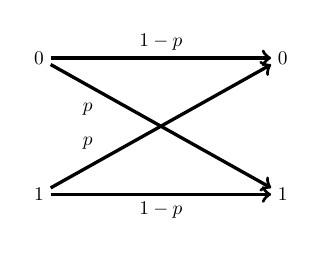
\begin{tikzpicture}[scale=0.7,transform shape]
        \node (zeroinput) {0};
        \node[below = 2cm of zeroinput] (oneinput) {1};
        \node[right = 4cm of zeroinput] (zerooutput) {0};
        \node[below = 2cm of zerooutput] (oneoutput) {1};
        \draw [->,very thick] (zeroinput) to node[above] {$1-p$} (zerooutput);
        \draw [->,very thick] (oneinput) to node[below] {$1-p$}  (oneoutput);
        \draw [->,very thick] (zeroinput) to  (oneoutput);
        \draw [->,very thick] (oneinput) to  (zerooutput);
        \node[above right = 0.65cm of oneinput] {$p$};
        \node[below right = 0.65cm of zeroinput] {$p$};
      \end{tikzpicture}
    \end{figure}
    \pause If the input is equally likely to be 0 or 1, are the input and output independent?
  \end{block}
  \normalsize
\end{frame}

%% Frame %%
\begin{frame}{Consequences of Independence}
  \footnotesize
  \begin{itemize}
    \item \pause If $X$ and $Y$ are independent, then the events $\{X \in A\}$ and $\{Y \in B\}$ are independent for any subsets $A$ and $B$ of $\mathbb{R}$
    \item \pause If $X$ and $Y$ are independent, then for any functions $g,h : \mathbb{R} \rightarrow \mathbb{R}$ the random variables $g(X)$ and $h(Y)$ are independent
    \item \pause Let $X$ and $Y$ be discrete random variables with probability mass functions $f_X(x)$ and $f_Y(y)$ respectively

    \pause Let $f_{X,Y}(x,y) = P\left(\{X =x\} \cap \{Y =y\} \right)$ be the joint probability mass function of $X$ and $Y$

    \pause $X$ and $Y$ are independent if and only if
      \begin{equation*}
        f_{X,Y}(x,y) = f_X(x) f_Y(y) \ \ \ \ \ \ \text{ for all } x,y \in \mathbb{R}
      \end{equation*}
  \end{itemize}
  \normalsize
\end{frame}

%% Frame %%
\begin{frame}{Continuous Random Variable}
  \footnotesize
  \begin{definition}
  \pause
    A random variable is called continuous if its distribution function can be expressed as
      \begin{equation*}
        F(x) = \int_{-\infty}^x f(u) \ du \ \ \text{for all} \ \ x \in \mathbb{R}
      \end{equation*}
    for some integrable function $f: \mathbb{R} \rightarrow [0,\infty)$ called the probability density function of $X$.
  \end{definition}
  \pause
  \begin{example}[Uniform Random Variable]
    A continuous random variable $X$ on the interval $[a,b]$ with cdf 
    \pause
    \begin{equation*}
      F(x) = \left\{\begin{array}{ll}
                    0, & \textsf{if $x < a$} \\
                    \frac{x-a}{b-a}, & \textsf{if $a \leq x \leq b$} \\
                    1, & \textsf{if $x > b$}
                   \end{array}
            \right.
    \end{equation*}
    \pause The pdf is given by
    \begin{equation*}
      \pause f(x) = \left\{
                      \begin{array}{cc}
                        \frac{1}{b-a} & \text{for } a \leq x \leq b \\
                        0 & \text{otherwise}
                      \end{array}
                    \right.
    \end{equation*}
  \end{example}
  \normalsize
\end{frame}

%% Frame %%
\begin{frame}{Probability Density Function Properties}
  \footnotesize
  \begin{itemize}
    \item \pause $F(a) = \pause \int_{-\infty}^{a} f(x) \ dx$
    \item \pause $P(a \leq X \leq b) =\pause  \int_{a}^{b}f(x) \ dx$
    \item \pause $\int_{-\infty}^{\infty} f(x)\ dx =\pause  1$
    \item \pause The numerical value $f(x)$ is not a probability. It can be larger than 1.
    \item \pause $f(x)dx$ can be intepreted as the probability $P(x < X \leq x + dx)$ \pause since
    \begin{equation*}
      P(x < X \leq x + dx) = F(x + dx) - F(x) \approx f(x) \ dx
    \end{equation*}
  \end{itemize}
  \normalsize
\end{frame}

%% Frame %%
\begin{frame}{Independent Continuous Random Variables}
  \footnotesize
  \begin{itemize}
    \item \pause Continuous random variables $X$ and $Y$ are independent if the events $\{X \leq x\}$ and $\{Y \leq y\}$ are independent for all $x$ and $y$ in $\mathbb{R}$
    \item \pause If $X$ and $Y$ are independent, then the random variables $g(X)$ and $h(Y)$ are independent
    \item \pause Let the joint probability distribution function of $X$ and $Y$ be $F(x,y) = P(X \leq x, Y \leq y)$.

    \pause Then $X$ and $Y$ are said to be jointly continuous random variables with joint pdf $f_{X,Y}(x,y)$ if
      \begin{equation*}
        F(x,y) = \int_{-\infty}^x \int_{-\infty}^y f_{X,Y}(u,v) \ du\ dv
      \end{equation*}
      for all $x,y$ in $\mathbb{R}$
    \item \pause $X$ and $Y$ are independent if and only if
      \begin{equation*}
        f_{X,Y}(x,y) = f_X(x) f_Y(y) \ \ \ \ \ \ \text{ for all } x,y \in \mathbb{R}
      \end{equation*}
  \end{itemize}
  \normalsize
\end{frame}

%% Frame %%
\begin{frame}{Expectation}
  \footnotesize
  \begin{itemize}
    \item \pause The expectation of a discrete random variable $X$ with probability mass function $f$ is defined to be
      \begin{equation*}
        E(X) = \sum_{x:f(x) > 0} xf(x)
      \end{equation*}
    \item \pause The expectation of a continuous random variable with density function $f$ is given by
      \begin{equation*}
        E(X) = \int_{-\infty}^\infty x f(x) \ dx
      \end{equation*}
    \item \pause If $a, b \in \mathbb{R}$, then $E(aX + bY) = aE(X) + bE(Y)$
    \item \pause If $X$ and $Y$ are independent, $E(XY) = E(X)E(Y)$
    \item \pause $X$ and $Y$ are said to be uncorrelated if $E(XY) = E(X)E(Y)$
    \item \pause Independent random variables are uncorrelated but uncorrelated random variables need not be independent
      \pause
      \begin{block}{Example}
        $Y$ and $Z$ are independent random variables such that $Z$ is equally likely to be $1$ or $-1$ and $Y$ is equally likely to be $1$ or $2$. \pause Let $X = YZ$. 
        
        \pause Then $X$ and $Y$ are uncorrelated but not independent.
      \end{block}
  \end{itemize}
  \normalsize
\end{frame}

%% Frame %%
\begin{frame}{Variance}
  \footnotesize
  \begin{itemize}
    \item \pause $\var(X) = \pause E\left[\left(X-E[X]\right)^2\right] \pause = E(X^2) - \left[ E(X)\right]^2$
    \item \pause For $a \in \mathbb{R}$, $\var(aX) = a^2\var(X)$
    \item \pause $\var(X+Y) = \var(X) + \var(Y)$ if \pause $X$ and $Y$ are uncorrelated
  \end{itemize}
  \normalsize
\end{frame}

%% Frame %%
\begin{frame}{Complex Random Variable}
  \footnotesize
  \pause
  \begin{definition}
    A complex random variable $Z=X+jY$ is a pair of real random variables $X$ and $Y$.
  \end{definition}
  \pause
  \begin{block}{Remarks}
    \begin{itemize}
      \item The cdf of a complex RV is the joint cdf of its real and imaginary parts.
      \pause
      \item $E[Z] = \pause E[X] + jE[Y]$
      \pause
      \item $\var[Z] = \pause E[\lvert Z \rvert^2] - \lvert E[Z] \rvert^2 = \pause \var[X] + \var[Y]$
    \end{itemize}
  \end{block}
  \normalsize
\end{frame}

%% Frame %%
\begin{frame}{}
\vfill
\begin{center}
Thanks for your attention
\end{center}
\vfill
\end{frame}


\end{document}
